\section{Настройка сети}

В машине Metasploitable2 выполним следующие команды для настройки сети:

\begin{lstlisting}[language=bash,caption={bash version}]
msfadmin@metasploitable:~$ sudo ip addr add 10.0.0.1/24 dev eth1
msfadmin@metasploitable:~$ sudo ip link set eth1 up
\end{lstlisting}

Проверим, что адрес успешно установился:

\begin{lstlisting}[language=bash]
1: lo: <LOOPBACK,UP,LOWER_UP> mtu 16436 qdisc noqueue 
link/loopback 00:00:00:00:00:00 brd 00:00:00:00:00:00
inet 127.0.0.1/8 scope host lo
inet6 ::1/128 scope host 
valid_lft forever preferred_lft forever
2: eth0: <BROADCAST,MULTICAST,UP,LOWER_UP> mtu 1500 qdisc pfifo_fast qlen 1000
link/ether 08:00:27:9a:98:38 brd ff:ff:ff:ff:ff:ff
inet 10.0.2.15/24 brd 10.0.2.255 scope global eth0
inet6 fe80::a00:27ff:fe9a:9838/64 scope link 
valid_lft forever preferred_lft forever
3: eth1: <BROADCAST,MULTICAST,UP,LOWER_UP> mtu 1500 qdisc pfifo_fast qlen 1000
link/ether 08:00:27:92:f0:ec brd ff:ff:ff:ff:ff:ff
inet 10.0.0.1/24 scope global eth1
inet6 fe80::a00:27ff:fe92:f0ec/64 scope link 
valid_lft forever preferred_lft forever
\end{lstlisting}

Адрес правильный. Теперь настроим сеть в Kali:

\begin{figure}[H]
	\centering
	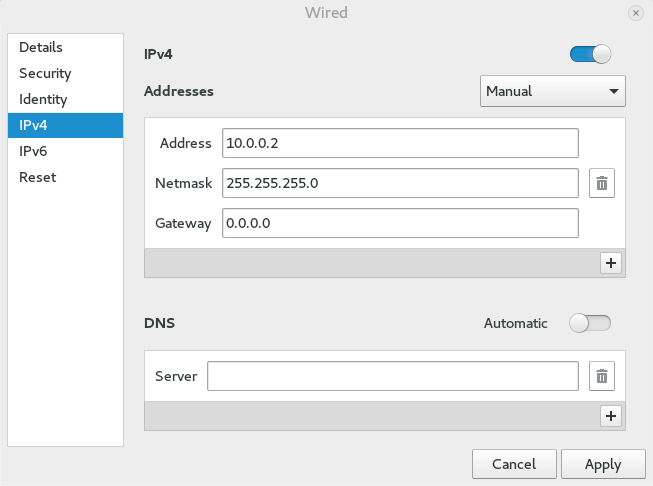
\includegraphics[width=0.7\textwidth]{nm1.png}
	\caption{Установка IPv4-адреса сети}
\end{figure}

Проверка:

\begin{figure}[H]
	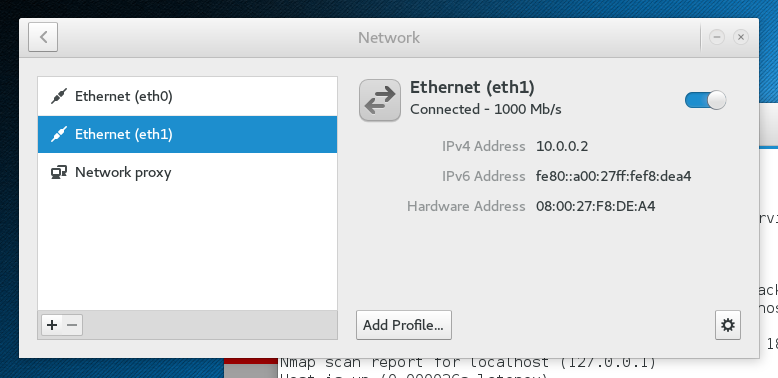
\includegraphics[width=\textwidth]{nm2.png}
	\caption{Состояние интерфейса}
\end{figure}

Так как в ходе работы придется читать много man-ов, настроим прокрутку в man-страницах (в пейджере по умолчанию, more, нельзя листать вверх).

\begin{lstlisting}[language=bash]
root@kali:~# export PAGER=less
\end{lstlisting}

\section{Сканирование сети}

Просканируем сеть:

\begin{lstlisting}[language=bash]
# nmap -sn 10.0.0.1/24

Starting Nmap 7.01 ( https://nmap.org ) at 2016-03-20 19:08 EDT
Nmap scan report for 10.0.0.1
Host is up (0.00023s latency).
MAC Address: 08:00:27:92:F0:EC (Oracle VirtualBox virtual NIC)
Nmap scan report for 10.0.0.2
Host is up.
Nmap done: 256 IP addresses (2 hosts up) scanned in 1.98 seconds
\end{lstlisting}

Просканируем порты:

\begin{lstlisting}[language=bash]
root@kali:~# nmap 10.0.0.1

Starting Nmap 7.01 ( https://nmap.org ) at 2016-03-20 15:34 EDT
Nmap scan report for 10.0.0.1
Host is up (0.00018s latency).
Not shown: 977 closed ports
PORT     STATE SERVICE
21/tcp   open  ftp
22/tcp   open  ssh
23/tcp   open  telnet
25/tcp   open  smtp
53/tcp   open  domain
80/tcp   open  http
111/tcp  open  rpcbind
139/tcp  open  netbios-ssn
445/tcp  open  microsoft-ds
512/tcp  open  exec
513/tcp  open  login
514/tcp  open  shell
1099/tcp open  rmiregistry
1524/tcp open  ingreslock
2049/tcp open  nfs
2121/tcp open  ccproxy-ftp
3306/tcp open  mysql
5432/tcp open  postgresql
5900/tcp open  vnc
6000/tcp open  X11
6667/tcp open  irc
8009/tcp open  ajp13
8180/tcp open  unknown
MAC Address: 08:00:27:92:F0:EC (Oracle VirtualBox virtual NIC)

Nmap done: 1 IP address (1 host up) scanned in 0.16 seconds
\end{lstlisting}

Анализ версий ПО:

\begin{lstlisting}[language=bash]
root@kali:~# nmap -sV 10.0.0.1

Starting Nmap 7.01 ( https://nmap.org ) at 2016-03-20 15:32 EDT
Nmap scan report for 10.0.0.1
Host is up (0.00018s latency).
Not shown: 977 closed ports
PORT     STATE SERVICE     VERSION
21/tcp   open  ftp         vsftpd 2.3.4
22/tcp   open  ssh         OpenSSH 4.7p1 Debian 8ubuntu1 (protocol 2.0)
23/tcp   open  telnet      Linux telnetd
25/tcp   open  smtp        Postfix smtpd
53/tcp   open  domain      ISC BIND 9.4.2
80/tcp   open  http        Apache httpd 2.2.8 ((Ubuntu) DAV/2)
111/tcp  open  rpcbind     2 (RPC #100000)
139/tcp  open  netbios-ssn Samba smbd 3.X (workgroup: WORKGROUP)
445/tcp  open  netbios-ssn Samba smbd 3.X (workgroup: WORKGROUP)
512/tcp  open  exec        netkit-rsh rexecd
513/tcp  open  login?
514/tcp  open  tcpwrapped
1099/tcp open  rmiregistry GNU Classpath grmiregistry
1524/tcp open  shell       Metasploitable root shell
2049/tcp open  nfs         2-4 (RPC #100003)
2121/tcp open  ftp         ProFTPD 1.3.1
3306/tcp open  mysql       MySQL 5.0.51a-3ubuntu5
5432/tcp open  postgresql  PostgreSQL DB 8.3.0 - 8.3.7
5900/tcp open  vnc         VNC (protocol 3.3)
6000/tcp open  X11         (access denied)
6667/tcp open  irc         Unreal ircd
8009/tcp open  ajp13       Apache Jserv (Protocol v1.3)
8180/tcp open  http        Apache Tomcat/Coyote JSP engine 1.1
MAC Address: 08:00:27:92:F0:EC (Oracle VirtualBox virtual NIC)
Service Info: Hosts:  metasploitable.localdomain, localhost, irc.Metasploitable.LAN; OSs: Unix, Linux; CPE: cpe:/o:linux:linux_kernel

Service detection performed. Please report any incorrect results at https://nmap.org/submit/ .
Nmap done: 1 IP address (1 host up) scanned in 13.54 seconds
\end{lstlisting}

\begin{figure}[H]
	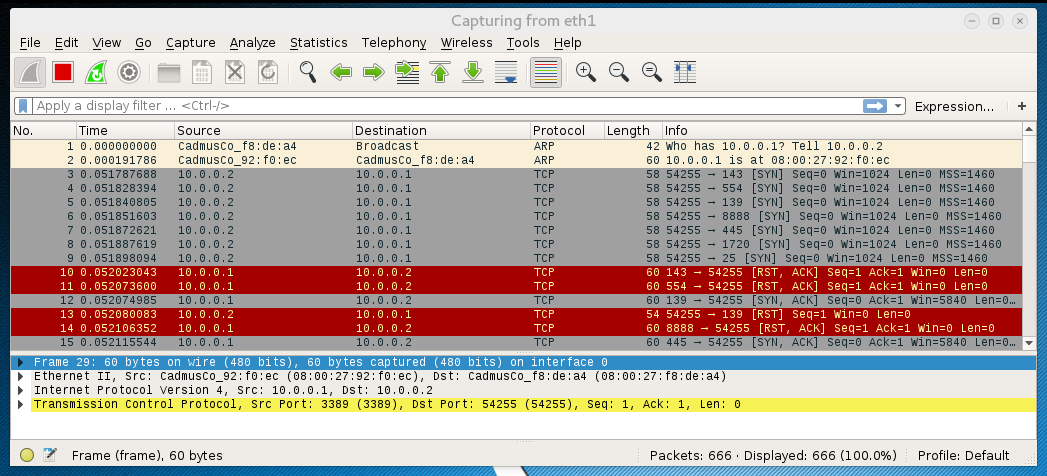
\includegraphics[width=\textwidth]{wireshark.png}
	\caption{Анализатор трафика Wireshark}
\end{figure}

\section{Анализ файлов Nmap}

Найдем файлы с БД:

\begin{lstlisting}[language=bash]
root@kali:~# dpkg -L nmap | grep services
/usr/share/nmap/scripts/snmp-win32-services.nse
/usr/share/nmap/nmap-services
root@kali:~# dpkg -L nmap | grep os-db
/usr/share/nmap/nmap-os-db
\end{lstlisting}

\section{Написание своего правила}

\begin{lstlisting}[language=bash]
root@kali:~# scp artyom@desktop:/mnt/win7/Users/Artyom/Documents/Study/Networks_new/Networks_10_11.zip .
artyom@desktop's password: 
Networks_10_11.zip                            100%   55KB  55.1KB/s   00:01    
root@kali:~# unzip Networks_10_11.zip 
\end{lstlisting}

\begin{lstlisting}[language=bash]
root@kali:~/Aleksyuk/CourseClient# ./main 
Please enter the command: Hi
You need to login first (AwesomeWallet 0.1)
\end{lstlisting}

Сделаем бекап файла с описанием отпечатков

\begin{lstlisting}[language=bash]
root@kali:~/Aleksyuk/CourseClient# sudo cp /usr/share/nmap/nmap-service-probes /usr/share/nmap/nmap-service-probes.backup
\end{lstlisting}

Напишем правило:

\begin{lstlisting}[language=bash]
root@kali:~# cat probe.txt 
Probe TCP AwesomeWallet q|\x02Hi|
rarity 1
ports 5004
match wallet m/^You need to login first \((\w*) ([\d.]*)\)/ p/$1/ v/$2/
\end{lstlisting}

Проверим работу регулярного выражения в Python:

\begin{lstlisting}[language=bash]
root@kali:~# python3
Python 3.5.1+ (default, Jan 13 2016, 15:09:18) 
[GCC 5.3.1 20160101] on linux
Type "help", "copyright", "credits" or "license" for more information.
>>> str = "You need to login first (AwesomeWallet 0.1)"
>>> import re
>>> p = re.compile(r"^You need to login first \((\w*) ([\d.]*)\)")
>>> m = p.match(str)
>>> print(m)
<_sre.SRE_Match object; span=(0, 43), match='You need to login first (AwesomeWallet 0.1)'>
>>> m.group()
'You need to login first (AwesomeWallet 0.1)'
>>> m.groups()
('AwesomeWallet', '0.1')
>>> exit()
\end{lstlisting}

Добавим правило:

\begin{lstlisting}[language=bash]
root@kali:~# cat probe.txt >> /usr/share/nmap/nmap-service-probes
\end{lstlisting}

Результат работы nmap:

\begin{lstlisting}[language=bash]
root@kali:~# nmap localhost -p 5004 -sV

Starting Nmap 7.01 ( https://nmap.org ) at 2016-03-20 18:24 EDT
Nmap scan report for localhost (127.0.0.1)
Host is up (0.000036s latency).
Other addresses for localhost (not scanned): ::1
PORT     STATE SERVICE VERSION
5004/tcp open  wallet  AwesomeWallet 0.1

Service detection performed. Please report any incorrect results at https://nmap.org/submit/ .
Nmap done: 1 IP address (1 host up) scanned in 6.52 seconds
\end{lstlisting}

По выводу сервера видно, что было произведено подключение и был отправлен тестовый запрос

\begin{lstlisting}[language=bash]
root@kali:~/Aleksyuk/Course# ./main 
Waiting
Connection 4
Waiting
Worker for 4 is up
Receiving message with length 2
Received Hi
Receiving message with length 2
Received 
Receiving message with length 2
Received 
ERROR writing to socket: Broken pipe
\end{lstlisting}

https://nmap.org/book/vscan-fileformat.html